\documentclass[a4paper,12pt,titlepage]{article}
\usepackage{kantlipsum}
\usepackage[paperwidth=0.5\paperwidth]{geometry}
% \usepackage{showframe}
\usepackage{graphicx}
\usepackage{changepage}
\usepackage{tikzpagenodes}

\usepackage{tikz}
\usetikzlibrary{calc}
\usetikzlibrary{decorations.pathmorphing}

\usepackage{fontspec}
\usepackage{hyperref}
\usepackage{microtype}
\setmainfont{Adobe Garamond Pro}

\geometry{top=1in, bottom=1in, left=1.5cm, right=1.5cm}

\setlength{\parindent}{0pt}

\begin{document}
% \maketitle

\begin{titlepage}
    \centering

    \begin{tikzpicture}[remember picture,overlay,
        shift={(current page.north west)}
    ]
    \node[anchor=north west,xshift=0.65cm,yshift=-0.65cm]{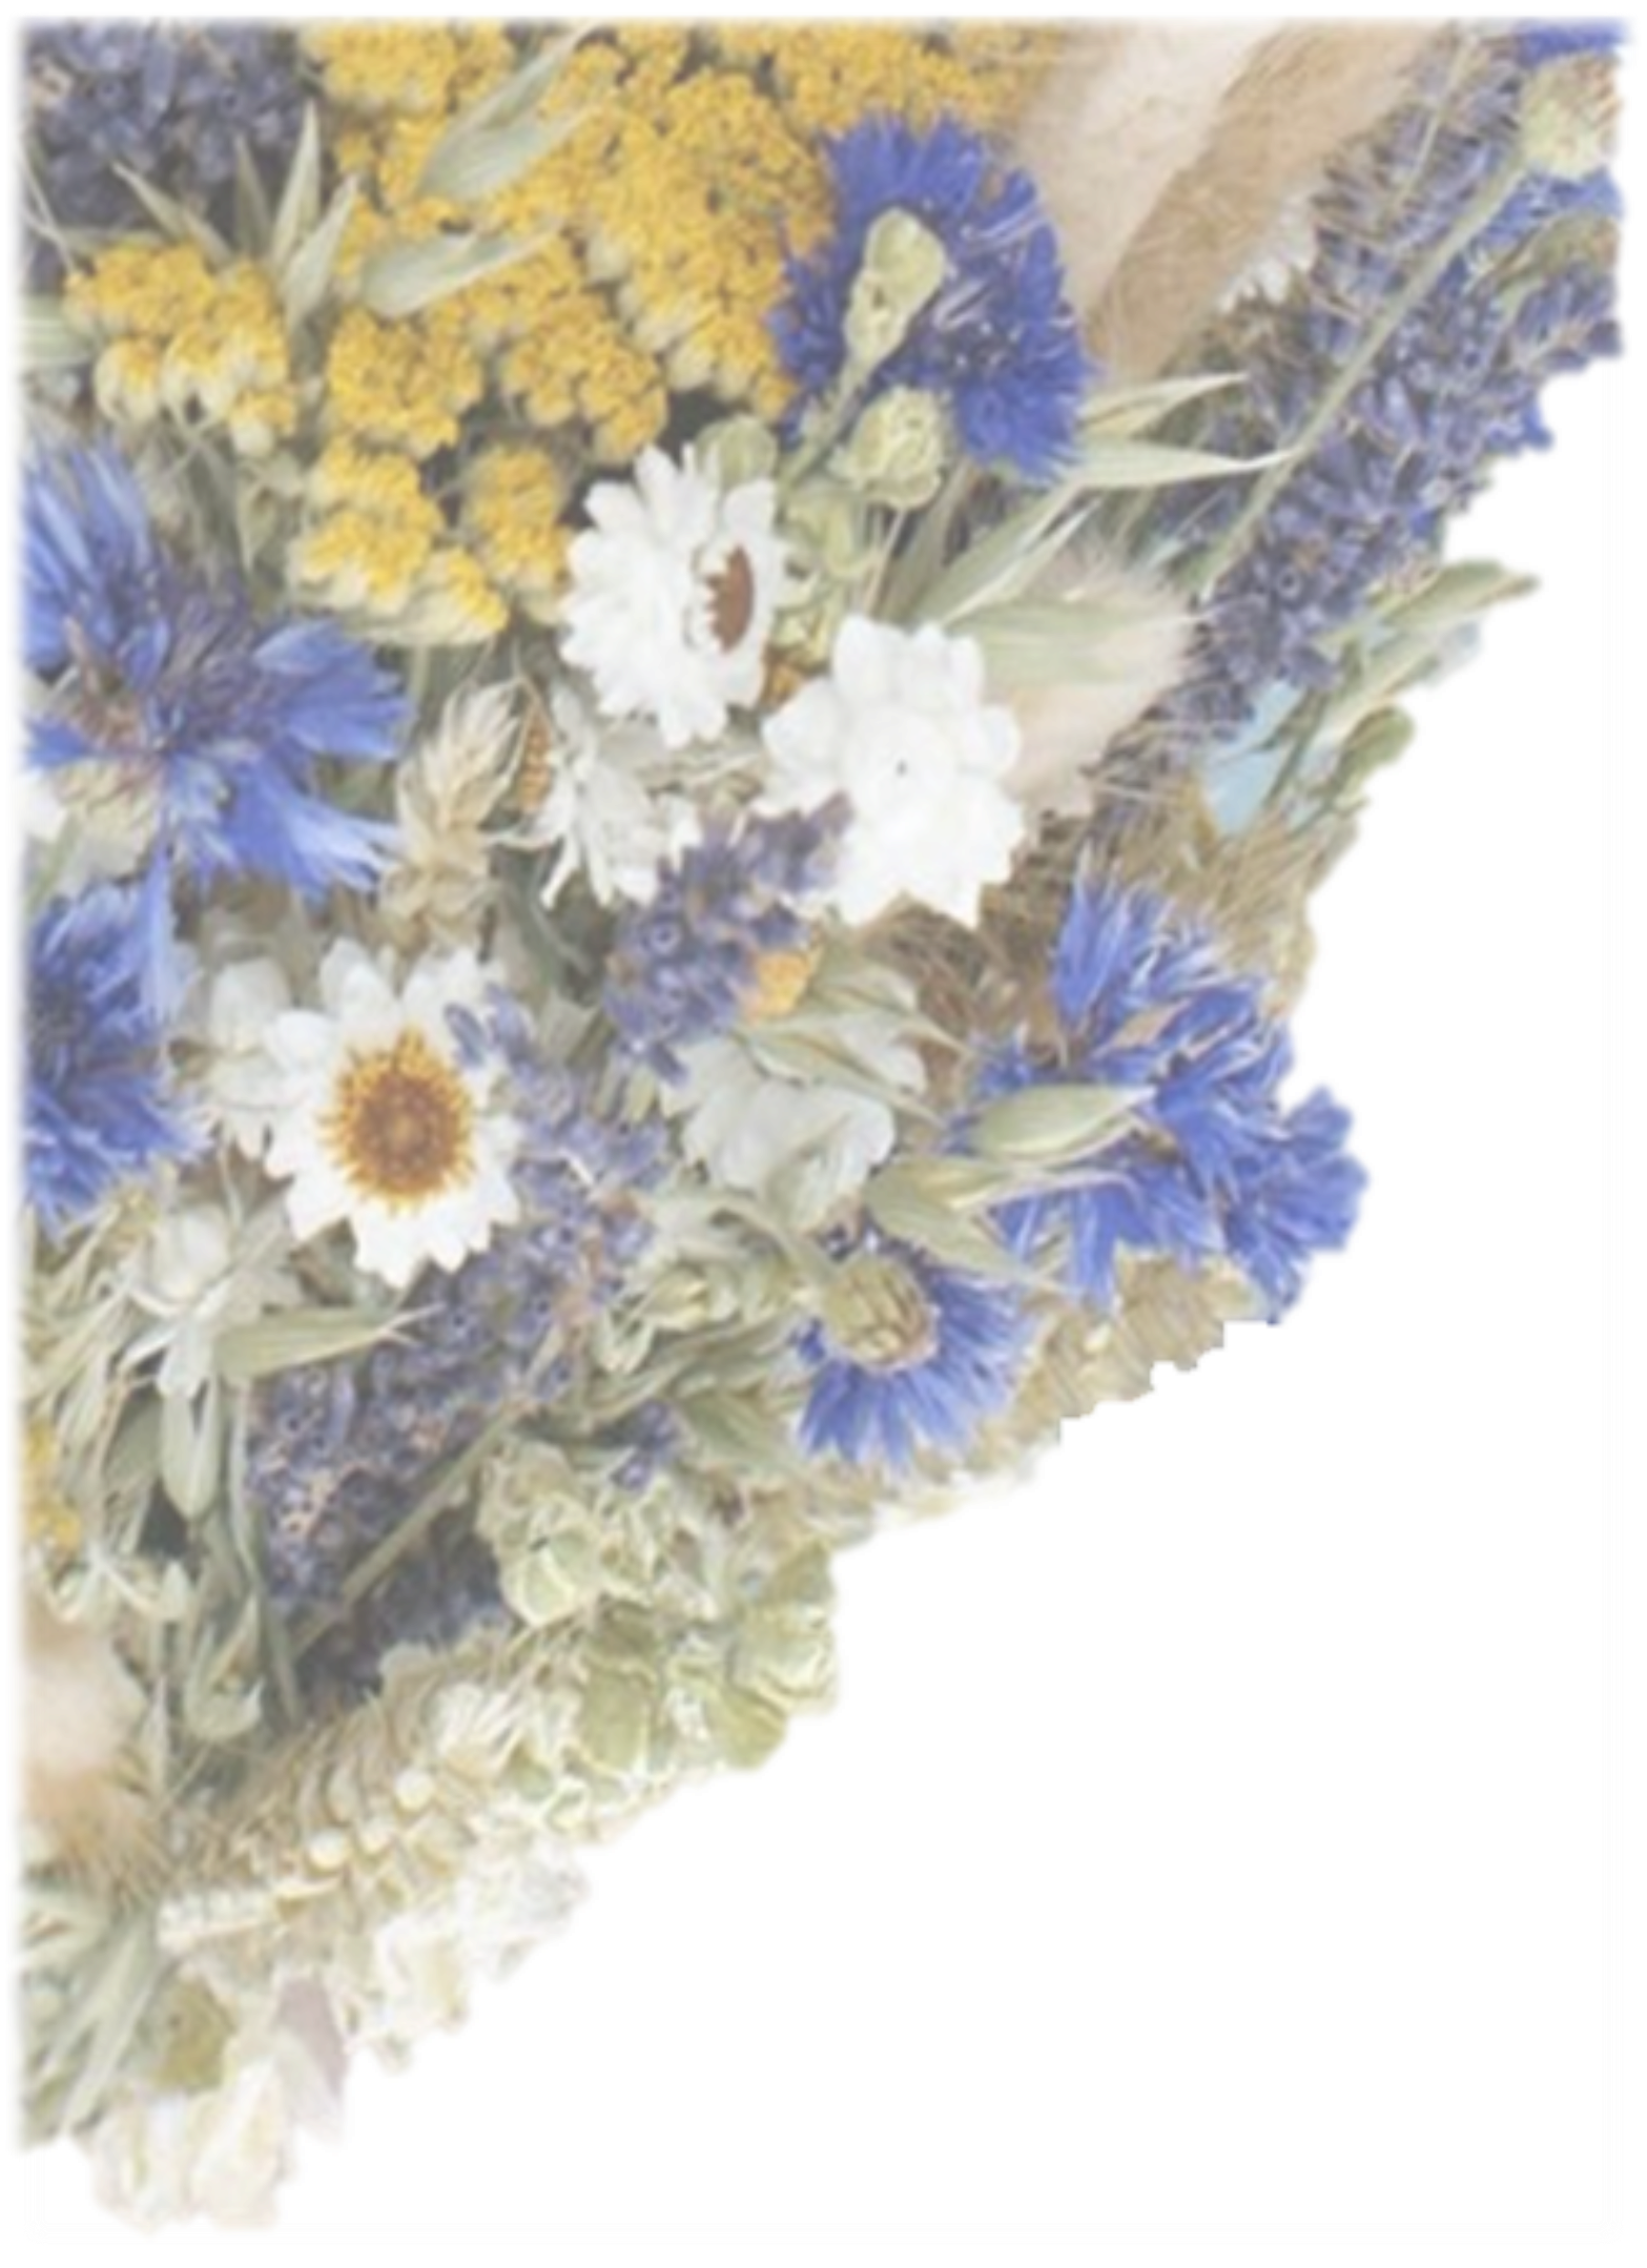
\includegraphics[width=0.3\paperwidth]{bouquet_edit3_transparent}};
    \end{tikzpicture}

    \begin{tikzpicture}[remember picture,overlay,
        shift={(current page.north east)}
    ]
    \node[xscale=-1,anchor=north west,xshift=0.65cm,yshift=-0.65cm]{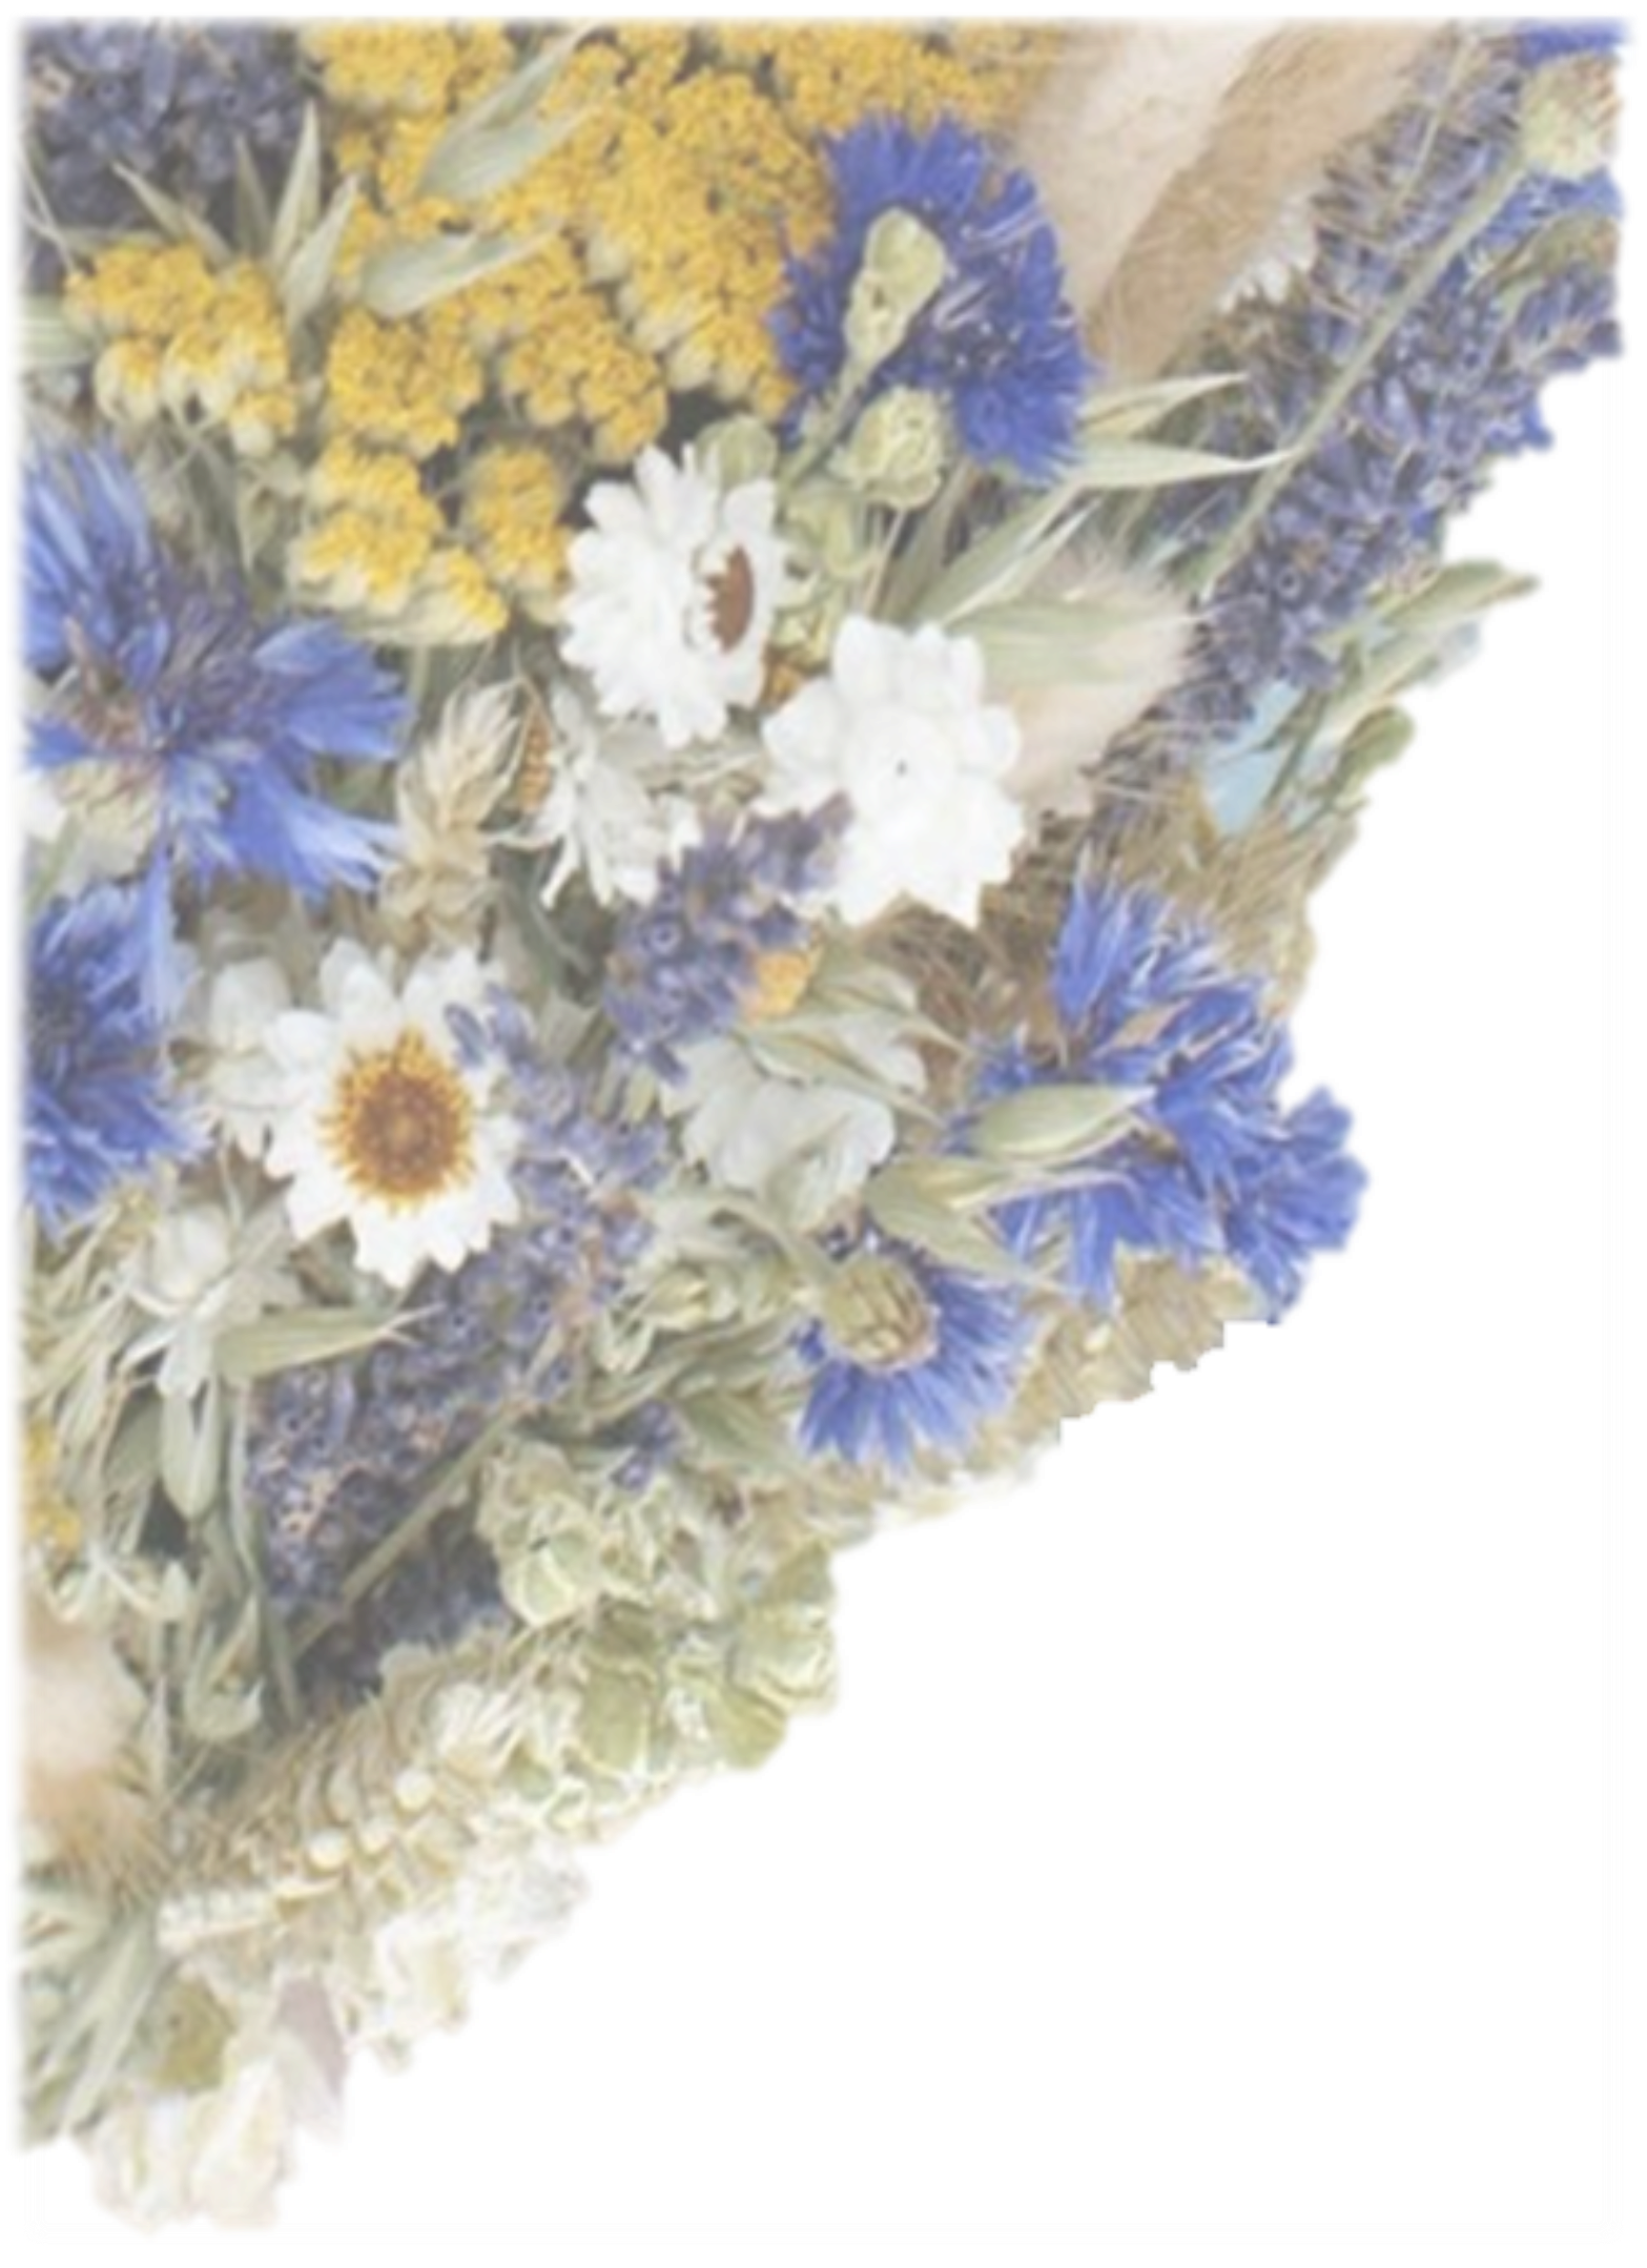
\includegraphics[width=0.3\paperwidth]{bouquet_edit3_transparent}};
    \end{tikzpicture}

    \begin{tikzpicture}[overlay,remember picture]
        \draw [line width=0.3mm,draw=black]
            ($ (current page.north west) + (0.6cm,-0.6cm) $)
            rectangle
            ($ (current page.south east) + (-0.6cm,0.6cm) $);
        \draw [line width=0.2mm,draw=black]
            ($ (current page.north west) + (0.8cm,-0.8cm) $)
            rectangle
            ($ (current page.south east) + (-0.8cm,0.8cm) $);
    \end{tikzpicture}
    
        
    \centering
    \vspace*{4.5cm}
    \begin{adjustwidth}{-2cm}{-2cm}
    \centering
    {\LARGE The Wedding of\\Dr. Rebecca Claire Brouwers\\{\em and}\\ Mr. Adam Alexander Harries\par}
    \end{adjustwidth}
	\vspace{2.5cm}
    {\large St.~Peter's Church, Lutton Place\par}
    {\large Rev.~Nick Wills\par}
    % \vspace{2.5cm}
    {\large September 19th, 2020\par}
	\vspace{3cm}
    
    \vspace{3cm}

\end{titlepage}

\hspace{2em}Welcome to St.~Peter's Church, Lutton place, and welcome to our wedding. We're delighted that you are able to join us today, despite the danger and frustration that these times have wreaked upon us. Our hope was always that we would celebrate our unity with as many of our friends and family as possible, but given the issues that would now pose, we are still delighted to be joined by the select group here today.

\hspace{2em}The reduced numbers are, sadly, not the only way that today's celebrations will differ from our original plans. Due to the various restrictions that are in place (legal, and otherwise) there will be no sung hymns during the service (though do please feel free to hum quietly and safely into your mask), and our reception will be considerably diminished and ``spread out'' over the coming few days.

\hspace{2em}Finally, we ask that all attendees make liberal use of the provided handwash, remain in your allocated seats, and take your favour bag (and contents) with you when you leave.

\begin{flushright}
Rebecca \& Adam
\end{flushright}

\vspace*{\fill}

{\em Entry of the Bride:} ``Hornpipe'' from {\em Water Music}, Suite in D major (HWV 349): George Frideric Handel.

\section{Greeting} 

Grace and peace to you from God our Father and the Lord Jesus Christ. \\

{\bf Amen.}

\clearpage

\section{Introduction} 
{\em President:} We have come together in the presence of God to witness the marriage of Rebecca and Adam, to celebrate their love for each other, and to ask God's blessing upon them.\\

Through the ages, people on great journeys have stopped at important places, and at decisive moments, to build cairns at the roadside to which they and others can always return.\\

Our life consists not only in being but also in becoming, it is a journey in which we grow and are transformed.\\

The great stories of God’s people and the coming of Jesus proclaim the faithfulness of God’s covenant and promise. God as Trinity (Father, Son and Holy Spirit) reveals to us the very nature of love in relationship. Relationships give human life its purpose and direction.\\

Rebecca and Adam's relationship is a great journey that, in different ways, we have travelled and will continue to travel with them. Today we pause along the way to gather at a decisive and important moment for us all. They are to be married.\\

We mark this decisive moment in Rebecca and Adam's journey now, adding to the cairn the stones of our love, our support and our prayers for them as they make their promises.\\

Creating and Redeeming God,\newline
it is your love which draws us together.\newline
Through the love which we have for one another,\newline
may we also grow in love for you.\newline
Walking with Christ as our companion on the way,\newline
may we come to share the joy\newline
which you have prepared for all who love you;\newline
through Jesus Christ our Lord.\newline\newline
{\bf Amen.}

\clearpage 

\section{Declarations of Intention}

{\em The president addresses Adam:}\\
Adam, do you give yourself to Rebecca in marriage? \\

{\em \hspace{2em} I do.} \\

Will you love her, respect her, and be for ever faithful to her? \\

{\em \hspace{2em} I will.}\\

{\em The president addresses Rebecca:} 

Rebecca, do you give yourself to Adam in marriage?\\

{\em \hspace{2em} I do.}\\

Will you love him, respect him, and be for ever faithful to him?\\ 

{\em \hspace{2em} I will.}\\

{\em The president addresses the families:}

Will you, the families of Rebecca and Adam, 
uphold and care for them in their life together?\\

{\bf \hspace{2em} We will.}\\

{\em The president addresses the congregation:}

Will all of you support and encourage Rebecca and Adam in their marriage?\\

{\bf \hspace{2em} We will.}\\

May God, who gave you the will to declare these intentions, give you also the 
grace to fulfil them.\\

{\bf Amen.}

\clearpage
\section{The Liturgy of the Word}

{\em Reading, Ayden Brouwers } - Luke 12: 22-31\\ 

{\bf \em Do Not Worry:}

Then Jesus said to his disciples: ``Therefore I tell you, do not worry about your life, what you will eat; or about your body, what you will wear. For life is more than food, and the body more than clothes. Consider the ravens: They do not sow or reap, they have no storeroom or barn; yet God feeds them. And how much more valuable you are than birds! Who of you by worrying can add a single hour to your life? Since you cannot do this very little thing, why do you worry about the rest?''

``Consider how the wild flowers grow. They do not labour or spin. Yet I tell you, not even Solomon in all his splendour was dressed like one of these. If that is how God clothes the grass of the field, which is here today, and tomorrow is thrown into the fire, how much more will he clothe you —- you of little faith! And do not set your heart on what you will eat or drink; do not worry about it. For the pagan world runs after all such things, and your Father knows that you need them. But seek his kingdom, and these things will be given to you as well.''\\

{\em Sermon, Rev.~Nick Wills}\\

{\em Those who are to be married stand in front of the president.}\\

{\em President:}\\ O God, whom to follow is to risk our whole lives: as Ruth and Naomi loved and held to one another, abandoning the ways of the past, so may Rebecca and Adam not be divided, but travel together into that strange land where you will lead us through Jesus Christ.\\

{\bf Amen.}

\clearpage
\section{The Promises}

{\em Rebecca and Adam face each other. Adam takes Rebecca's right hand and says:}

Before God and our friends, I, Adam, give myself to you, Rebecca, in loving and lifelong marriage. I promise to be with you, in sorrow and in joy, in need and in plenty, in frailty and in strength. God keep me always true to this promise.\\

{\em They loose hands. Rebecca takes Adam's right hand and says:}

Before God and our friends, I, Rebecca, give myself to you, Adam, in loving and lifelong marriage. I promise to be with you, in sorrow and in joy, in need and in plenty, in frailty and in strength. God keep me always true to this promise.\\

{\em They loose hands.}

\section{The Giving and Receiving of Rings}

{\em Rebecca and Adam face each other.}\\

{\em Adam places a ring on Rebecca's finger, saying:}\\
Rebecca, I give you this ring as I give you myself, all that I have, and all that I am.\\

{\em Rebecca places a ring on Adam's finger, saying:}\\
Adam, I give you this ring as I give you myself, all that I have, and all that I am.

\clearpage
\section{The Proclamation}

{\em As Rebecca and Adam continue to face each other, joining hands, the congregation says:}\\
{\bf We have witnessed the promises of Rebecca and Adam.
Together we now handsel\footnote{`Handsel' - an old Scots word, meaning 'a gift bestowed to commemorate an inaugural occasion, event or season'.} them.\\
As they are pledged to each other in love, so we promise, in hope, to be a living sign of love in the world.}\\

{\em The president says to Rebecca and Adam:}\\
Rebecca and Adam, now that you have made these promises before God and before those gathered here, I declare that you are joined in marriage.\\

{\em (Applause is most welcome at this point!)} \\ 

The peace of the Lord be with you.

\section{The Peace}

{\em The president says to the congregation:}\\
We meet in Christ's name.\\

{\em The congregation responds:}\\
{\bf Let us share his peace.}\\

All may exchange a sign of peace.\\

{\em We request that all signs are non-contacting, and socially distanced.}

\section{The Registration} 

{\em The Registration takes place, in the sight of the congregation, at this point. Please be patient while the register is signed by the parties involved, and enjoy the music played by our wonderful organist Sheila Chisholm.}\\
\\
{\em Music:} An arrangement of selected hymns, including ``Amazing Grace'', ``Morning has broken'' and ``Tell out my soul''.

\clearpage
\section{The Prayer of \\Thanksgiving and Blessing}

{\em The President says:}\\
God of love and faithfulness, you give joy to bridegroom and to bride.\\
Uphold Rebecca and Adam in their marriage\\
and enfold them in your peace.\\
Give them wisdom and understanding\\
and sustain them in sickness and sorrow.\\
Teach them, throughout their life together,\\
the power of your promise, “You are blest.”\\


Rebecca and Adam, the blessing of God be upon you,\\
that good may come to you;\\
the blessing of Christ be upon you,\\
that good be done to you;\\
the blessing of the Holy Spirit be yours,\\
that good may be the course of your life,\\
each day of your arising, each night of your lying down,\\
for evermore.\\

{\bf Amen.}\\

As our Saviour Christ has commanded and taught us, we are bold to say:\\

{\bf Our Father,\\
who art in heaven,\\
hallowed be thy name;\\
thy kingdom come;\\
thy will be done;\\
on earth as it is in heaven.\\
Give us this day our daily bread;\\
and forgive us our trespasses,\\
as we forgive those\\
who trespass against us.\\
And lead us not into temptation,\\
but deliver us from evil.\\
For thine is the kingdom,\\
the power and the glory,\\
for ever and ever.\\
Amen.}

\clearpage
\section{Conclusion}

{\em President:} God of all the world, as you have called together Rebecca and Adam, so we have come together in your love.\\
 
As in your presence, Rebecca and Adam have promised to love each other, so we have promised to support them.\\

As Rebecca and Adam have declared their love for each other, may they declare your love for all the world.\\

As you have blessed Rebecca and Adam in their marriage, bless us now in our lives.
Make us, like them, a blessing to one another and to you. \\

Christ go before us to guide our steps\\
Christ be within us to kindle our vision\\
Christ shine from us to give joy to the world.\\

{\em The newly-married lead the congregation from the church.}\\

{\em Recessional music:} ``Toccata'' from Charles Marie Widor's 5th Organ Symphony.


\clearpage 


{\bf Thanks:}

\hspace{2em} We'd like to thank a few important people for helping to make our wedding happen, and supporting us along the way.


\hspace{2em} Firstly, of course, we'd like to thank those at the Church who have had such key roles in the ceremony: Rev.~Nick Wills, our Rector, Sheila Chisholm, the Organist, and Liz for assistance with the church flowers. 


\hspace{2em} We would also like to thank Chris Harries for agreeing to be the Best Man (and signing the schedule), Ayden Brouwers for his excellent reading, and Melanie Jutton for her unerring support, and for also being a signatory of the schedule. 

\hspace{2em} Our orignial conception of a socially distanced reception, and our restricted family reception, would not be possible without the assistance of Mary-Jane Brouwers, as well as Hugh, who also very kindly provided his car as our wedding carriage. 

\hspace{2em} Finally, we would like to thank all of you for attending, despite the danger that this brings to some of you, and for helping us to stay safe while celebrating our love in these turbulent times. 

\clearpage

\begin{center}
    \vspace*{\fill}
    {\centering \tiny
    This page unintentionally left blank.
    }    
    \vspace*{\fill}
\end{center}


\thispagestyle{empty}
 


\end{document}